% Apresenta a fundamentação teórica dos conceitos usados no trabalho. Pode haver mais de 
% uma seção tratando da fundamentação, se houver a necessidade de se tratar outros assuntos, 
% exemplo: trabalhos relacionados, ferramentas, bibliotecas, hardware e outros.

\section{Fundamentação teórica}

A gama de aplicações processo de inpainting em imagens digitais é ampla, uma vez que não se limita a um único domínio. A técnica pode ser aplicada em diversas áreas, tais como a medicina, engenharia, arquitetura, entre outras, as quais serão mais exploradas mais a fundo no tópico \ref{applications}.
Além disso, o conceito de inpainting, inicialmente apresentado em \ref{introduction}, não agrega apenas as ideias de restauração de imagens ou remoção de objetos, mas também a construção e reconstrução de imagens \cite{you2019pirec}, a preservação da privacidade (por exemplo, borramento de rostos e placas de veículos automotivos) em imagens públicas \cite{google2022magritte}, ao preenchimento de lacunas em imagens de satélites \cite{Maalouf2009bandelet}, entre outros possíveis usos, aos quais alguns serão mais explorados no prosseguir desta revisão. Por fim, o tópico \ref{related} apresenta os trabalhos relacionados ao tema. 

Neste trabalho, o escopo de inpainting de imagens pode ser compreendido como uma técnica utilizada para preencher regiões vacantes ou danificadas em uma imagem digital. O objetivo do inpainting é reconstruir as regiões afetadas de forma que o resultado final seja o mais visualmente plausível possível, ou seja, que a imagem resultante seja natural à ótica humana e não apresente artefatos visuais, enquanto preserva a coerência e consistência da imagem original \cite{levin2003learning}.

Há diversas formas de se implementar o processo de inpainting, sendo que a escolha do método a ser utilizado depende do domínio de aplicação, das características da imagem, do tipo de máscara, entre outros fatores \cite{black2020evaluation}. Contudo, é comum distinguir duas variedades de métodos amplamente utilizados: os métodos "clássicos", os quais geralmente utilizam informações da estrutura ou da imagem ou outras regiões para preencher lacunas, e os métodos baseados em aprendizado, os quais comumente utilizam grandes quantidades de dados para serem treinados, sendo que os métodos baseados em aprendizado são os mais recentes e apresentam geralmente resultados mais satisfatórios.


\subsection{Métodos clássicos} \label{patch}
Os métodos clássicos utilizam informações dos pixels e da região vizinha das regiões que estão vacantes ou danificadas para preencher as lacunas. Estes métodos são baseados no princípio de que regiões próximos e similares ao alvo são os mais adequados para preencher a região \cite{patchmatch2009, Bertalmio2001navier}. É possível ainda, dentro desta estratégia, distinguir dois tipos de métodos: os métodos baseados em patches, tais que utilizam amostras próximas da região-alvo para preencher a lacuna, e os métodos baseados em síntese de textura que utilizam a textura das regiões conhecidas para preencher a lacuna.

\begin{list}{}{}


  \item \textbf{Métodos baseados em difusão:} \label{diffusion}
Segundo \cite{black2020evaluation}, estes métodos transmitem os valores dos pixels adjacentes para as regiões a serem preenchidas e suas implementações são variadas. Métodos como \cite{Telea2004} utilizam uma o Método da Marcha Rápida, que consiste em propagar médias ponderadas das intensidades dos pixels adjacentes para a região-alvo, mantendo as altas e baixas frequências. Há outras implementações como \cite{Bertalmio2001navier}, que utilizam as equações de Navier-Stokes para a difusão de valores de pixels adjacentes ou até os isótopos das imagens. Estes métodos são simples e eficientes computacionalmente, porém, geralmente apresentam resultados com artefatos visuais, como bordas irregulares, texturas deformadas, etc, em especial, para imagens com texturas complexas.

  \item \textbf{Métodos baseados em patches:} \label{sample}
estes métodos utilizam amostras de regiões conhecidas e similares a região-alvo para reconstruí-la. Assume-se que a região corrompida possui pixels semelhantes a alguma área próxima, então o método seleciona uma amostra da área próxima e a transfere para a região-alvo, mantendo a coerência da imagem e a consistência da textura. Essa estratégia é simples e eficiente computacionalmente, em especial para imagens com texturas e estruturas simples \cite{patchmatch2009}, apesar de apresentarem resultados superiores aos de difusão. Contudo, não produz resultados satisfatórios para lidar com imagens mais compostas, como imagens com texturas complexas, imagens com bordas irregulares, imagens com objetos com texturas semelhantes, etc.

\item \textbf{Métodos baseados em síntese de textura:} \label{texture}
 estes métodos estão incluídos na categoria de métodos baseados em patches, pois também utilizam amostras de regiões conhecidas e similares a região-alvo para reconstruí-la. Contudo, estes métodos utilizam amostras de texturas para sintetizar novos pixels para a região-alvo. Estes métodos são baseados no princípio de que a textura de uma região é uma função de sua vizinhança, e assume que a área vizinha ao alvo possui texturas semelhantes, o que viabiliza propagar as bordas e frequências para preenchimento. Utilizar esta estratégia pode produzir resultados satisfatórios para imagens com texturas complexas, embora ainda encontrem dificuldades para lidar com imagens com bordas ou padrões irregulares, imagens com objetos com texturas semelhantes, entre outras \cite{bertalmio2003texture}.
\end{list}

% WRITE MORE ABOUT SUB TOPICS

\subsection{Métodos baseados em aprendizado} \label{learn-based}
Os métodos baseados em aprendizado, no que lhe concernem, utilizam técnicas de aprendizado de máquina, como redes neurais convolucionais (CNNs) e redes generativas adversárias (GANs) para preencher a região danificada. Estas técnicas "aprendem" a reconstruir a região danificada a partir de um conjunto de dados de imagens com e sem máscara. Estes métodos são mais recentes e apresentam resultados mais satisfatórios, em especial para imagens com texturas complexas, imagens com bordas irregulares, imagens com objetos com texturas semelhantes, etc. Contudo, estes métodos são mais complexos e computacionalmente mais custosos, devido ao fato que eles necessitam de um grande conjunto de dados para serem treinados \cite{Goodfellow-et-al-2016}.

\begin{list}{}{}
\item \textbf{Redes neurais convolucionais:} \label{cnn-based-learning}
utilizam uma CNN para reconstruir as regiões faltantes. Estes métodos se beneficiam da habilidade das CNNs de aprender as características de uma imagem e conseguem produzir bons resultados para imagens com texturas e estrutura complexas. A rede é treinada em um vasto conjunto de dados de imagens e aprende a reconhecer padrões e as características das imagens. Após o treinamento, a rede utiliza o conhecimento adquirido para gerar novos pixels para a região danificada, ainda preservando a região que a cerca.

\item \textbf{Redes generativas adversárias:} \label{gan-based-learning}
utilizam uma GAN para gerar novos pixels para preencher a região danificada. As GANs consistem em duas partes: uma rede geradora que gera novos pixels, e um discriminador que avalia a qualidade dos pixels obtidos\cite{black2020evaluation}. Estes métodos podem gerar resultados mais realísticos do que os baseados em CNNs, mas eles são mais custosos computacionalmente e requerem um conjunto de dados maior para treinamento. Consequentemente, estes métodos são mais complexos e costumam levar mais tempo para treinamento \cite{pathakCVPR16context}.

\end{list}
Em suma, o inpainting de imagem é uma técnica utilizada para preencher regiões faltantes ou corrompidas de uma imagem, como uma nuvem em uma imagem de sensoriamento remoto, ou danos causados pela degradação em fotografias digitalizadas, como na Figura \ref{fig:inpainting-couple}.
\begin{figure}[ht]
\centering
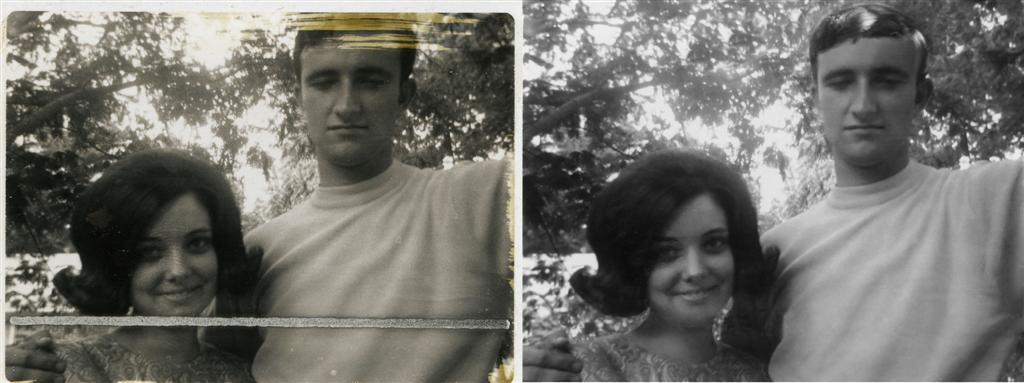
\includegraphics[width=1\textwidth]{inpainting-couple.jpg}
\caption{Exemplo do inpainting de imagens \cite{wiki:inpainting-couple}. A imagem da esquerda mostra uma imagem danificada. A imagem da direita mostra a imagem após o processo de inpainting.}
\label{fig:inpainting-couple}
\end{figure}


\subsubsection{Redes neurais convolucionais} \label{cnn}
\textbf{Definição} \label{cnn-def}
\textbf{Arquitetura} \label{cnn-arch}
\textbf{Treinamento} \label{cnn-train}
\textbf{Teste} \label{cnn-test}
\textbf{Erros} \label{cnn-err}
\textbf{Aplicações} \label{cnn-app}
\textbf{Limitações} \label{cnn-lim}
\textbf{Melhorias} \label{cnn-impr}

\subsubsection{Redes generativas adversárias} \label{gan}
\textbf{Definição} \label{gan-def}
\textbf{Arquitetura} \label{gan-arch}
\textbf{Treinamento} \label{gan-train}
\textbf{Teste} \label{gan-test}
\textbf{Erros} \label{gan-err}
\textbf{Aplicações} \label{gan-app}
\textbf{Limitações} \label{gan-lim}
\textbf{Melhorias} \label{gan-impr}


\subsubsection{Depth Inpainting} \label{quality-depth}
O Depth Inpainting é uma técnica utilizada para realizar o inpainting de imagens 3D, como é o caso de imagens obtidas por câmeras fotográficas ou sistemas de visão computacional. Esta técnica é útil em situações onde a câmera é incapaz de capturar corretamente as informações de profundidade, como é o caso de objetos translúcidos ou afetados pela luz especular (reflexos) \cite{shish20203dphoto}.

A técnica de Depth Inpainting consiste em utilizar uma rede neural convolucional para estimar a profundidade de uma imagem, treinada com imagens com values conhecidos, e então utilizar esta estimativa para realizar o inpainting da imagem-alvo. Outra abordagem é utilizar técnicas de processamento de imagens, como a interpolação de valores, para aproximar os values da região a ser preenchida. \cite{shish20203dphoto} Isto pode ser obtido analisando os padrões e estruturas dos pixels vizinhos. Em ambos casos, o algoritmo precisa ser treinado com uma base de dados de imagens com valores de profundidade conhecidos para aprender a realizar predições.



\subsection{Otimizações dos resultados}

% \subsubsection{Estrutura da imagem} \label{quality-struct}
\subsubsection{Patch-based inpainting} \label{quality-patch}


% \subsubsection{Edge-preserving inpainting} \label{quality-edge}
% \subsubsection{Priorização de regiões} \label{quality-prio}

\subsubsection{Preenchimentos intra e inter imagem} \label{quality-intra-inter}


\subsubsection{Inpainting guiado} \label{quality-guided}
A escolha da região a ser preenchida é parte fundamental na qualidade do resultado do processo de inpainting, uma vez que ela afeta diretamente a qualidade da imagem gerada. A região selecionada deve abranger a quantidade necessária para prover contexto suficiente para o algoritmo de inpainting, mas não deve ser muito grande, pois isso pode levar a resultados com texturas e estruturas não realistas ou com maior tempo de processamento. Ademais, a região escolhida deve ser bem definida e conter uma delimitação clara, para que o algoritmo de inpainting possa identificar com facilidade a região e estruturas a serem preenchidas \cite{huang2014image}. Alguns métodos realizam este processo de forma automática, sendo conhecidos como Blind Inpainting \cite{wang2020vcnet}.

Por seguinte, é importante ponderar a situação da região a ser preenchida no contexto da imagem, pois o processo de correção pode afetar a coerência do resultado, isto é, o preenchimento de uma região no conteúdo principal de uma imagem possui mais impacto ao comparar-se com o preenchimento de uma região de fundo.

A Figura \ref{fig:inpainting-region} mostra um exemplo da seleção de regiões para o processo de inpainting.
\begin{figure}[ht]
\centering
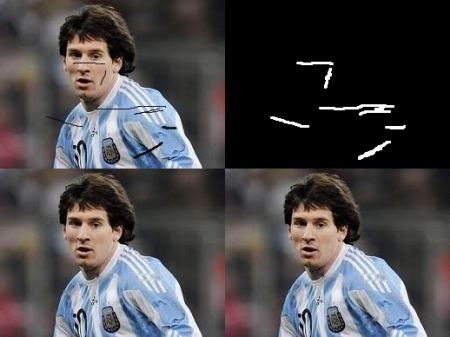
\includegraphics[width=0.8\textwidth]{inpainting-region.jpg}
\caption{Exemplo da seleção de regiões a serem preenchidas \cite{OpenCVmessi}. A imagem no canto superior esquerdo é a imagem danificada. No canto superior direito há a máscara (região) que selecionada pelo usuário para ser preenchida. A imagem no canto inferior esquerdo mostra a imagem após o processo de inpainting utilizando \cite{Bertalmio2001navier}, e a imagem no canto inferior direito mostra a imagem após o processo de inpainting utilizando \cite{Telea2004}.}
\label{fig:inpainting-region}
\end{figure}

\subsubsection{Context-aware inpainting} \label{quality-context}
\subsubsection{Representação esparsa} \label{quality-sparse}



\subsection{Otimizações computacionais}
\subsubsection{Profiling} \label{time-prof}
\subsubsection{Aceleração de hardware} \label{time-acel}
\subsubsection{Crop} \label{time-crop}
\subsubsection{Redução de memória} \label{time-mem}
\subsubsection{Paralelismo} \label{time-par}
\subsubsection{Estruturas de dados} \label{time-struct}
\subsubsection{Redução de redundância} \label{time-redund}
\subsubsection{Otimização de acesso a memória} \label{time-access}
\subsubsection{Vetorialização} \label{time-vect}
\subsubsection{Aproximações} \label{time-approx}
\subsubsection{Cálculos incrementais} \label{time-dist}


\subsection{Aplicações} \label{applications}

